\chapter{New Algorithms for Social Recommendation}

After studying the results of the first trial, we made use of what we learned to come up with new algorithms for social collaborative filtering. Our goal in designing these algorithms was to address deficiencies in current SCF methods that we pointed out in the Introduction chapter:

\begin{itemize}
\item {Non-feature-based user similarity}
% Note: potential for latent item information diffusion here
\item { Modeling direct user-user information diffusion}
\item { Restricted common interests}
\end{itemize}

\section{New Objective Components}

Again, the new algorithms each form a component of a minimization objective $Obj$ which is composed of sums of one or more objective components:

\begin{align}
\mathit{Obj} = \sum_i \lambda_i \mathit{Obj}_i
\end{align}

A sigmoidal transform 
\begin{align}
\sigma(o) & = \frac{1}{1 + e^{-o}}
\end{align}
of regressor outputs $o \in \R$ is used to squash the outputs 
to the range $[0, 1]$.  
In places where the $\sigma$ transform may be optionally included, 
this is written as $[\sigma]$.  

\subsection{Hybrid Objective}

As specified in Chapter 1, one weakness of  MF methods is that they cannot model joint features over user and items, and hence the cannot model direct user-user information diffusion. We fix this by introducing another objective component in addition to the standard MF objective, and this component serves as a simple linear regressor for such information diffusion observations. The resulting hybrid objective component becomes a combination of latent MF and linear regression objectives.

We make use of the $\f_{\x,\y}$ features to make the linear regressor. Using $\la \cdot,\cdot \ra$ to denote an inner product, we define a weight
vector $\w \in \R^F$ such that $\la \w, \f_{\x,\y} \ra = \w^T \f_{\x,\y}$ is the prediction of the system. The objective of the linear regression component is therefore

\begin{align*}
\sum_{(\x,\y) \in D} \frac{1}{2} (R_{\x,\y} - [\sigma] \w^T \f_{\x,\y})^2
\end{align*}

We combine the output of the linear regression objective with the Matchbox output $[\sigma] \x^T U^T V y$, to get a hybrid objective component. The full objective function for this hybrid model is

\begin{align}
\sum_{(\x,\y) \in D} \frac{1}{2} (R_{\x,\y} - [\sigma] \w^T \f_{\x,\y} - [\sigma] \x^T U^T V y)^2
\end{align}

\subsection{Social Spectral Regularization}

As we did with the Social Regularization method in Section~\ref{sec:SocRec}, we build on ideas used in Matchbox~\cite{matchbox} to extend social spectral regularization~\cite{sr,rrmf} by incorporating user features into the objective. 

\begin{align}
\sum_{\x} & \sum_{\z \in \mathit{friends}(\x)} \frac{1}{2} S^+_{\x,\z} \| U\x - U\z \|_2^2 \nonumber \\
& = \sum_{\x} \sum_{\z \in \mathit{friends}(\x)} \frac{1}{2} S^+_{\x,\z} \| U (\x - \z) \|_2^2 \nonumber \\
& = \sum_{\x} \sum_{\z \in \mathit{friends}(\x)} \frac{1}{2} S^+_{\x,\z} (\x - \z)^T U^T U (\x - \z)
\end{align}

\subfive Note: standard spectral regularization assumes $S^+_{\x,\z} \in [0,1]$;
however we may also want to try $S_{\x,\z}$ since a negative value actively
encourages the latent spaces to oppose each other, which may be desired.

\subsection{Social Co-preference Regularization}

A crucial aspect missing from other SCF methods is that while two users may not be globally similar or opposite 
in their preferences, there may be sub-areas of their interests which can be correlated to each other.
For example, two friends may have similar interests concerning music, but 
different interests concerning politics.  The social co-preference regularizers
aim to learn such selective co-preferences. The motivation is to constrain users $\x$
and $\z$ who have similar or opposing
preferences to be similar or opposite in the same latent latent space
relevant to item $\y$.  

We use $\la \cdot, \cdot \ra_{\bullet}$ to denoe a reweighted inner product. The objective component for 
social co-preference regularization along with its expanded form is

\begin{align}
\sum_{(\x,\z,\y) \in C} & \frac{1}{2} (P_{\x,\z,\y} - \la U\x, U\z \ra_{V\y})^2 \nonumber \\
& = \sum_{(\x,\z,\y) \in C} \frac{1}{2} (P_{\x,\z,\y} - \x^T U^T \diag(V\y) U \z)^2
%= & \sum_{(\x,\z,\y) \in C}  \frac{1}{2} (P_{\x,\z,\y} - \sum_{k=1}^K (U\x)_k (U\z)_k (V\y)_k )^2 
\end{align}


\subsection{Social Co-preference Spectral Regularization}
This is the same as the social co-preference regularization above, except that it uses the spectral regularizer format for 
learning the co-preferences.

 We use $\| \cdot \|_{2,\bullet}$ to denote a re-weighted $L_2$ norm. The objective component for
 social co-preference spectral regularization along with its expanded form is
 
\begin{align}
\sum_{(\x,\z,\y) \in C} & \frac{1}{2} P_{\x,\z,\y} \| U\x - U\z \|_{2,V\y}^2 \nonumber \\
& = \sum_{(\x,\z,\y) \in C} \frac{1}{2} P_{\x,\z,\y} \| U (\x - \z) \|_{2,V\y}^2 \nonumber \\
& = \sum_{(\x,\z,\y) \in C} \frac{1}{2} P_{\x,\z,\y} (\x - \z)^T U^T \diag(V\y) U (\x - \z)
%= & \sum_{\x} \sum_{\z \neq \x} \sum_{\y} \frac{1}{2} P_{\x,\z,\y} \sum_{k=1}^K \big( \left[ (U\x)_k - (U\z)_k \right] (V\y)_k \big)^2
\end{align}

\subsection{Derivatives}
As before, we seek to optimize sums of the above objectives and will use
gradient descent for this purpose. We again use the following useful abbreviations:

\begin{align*}
\s & = U \x \qquad \s_{k} = (U \x)_{k}; \; k=1\ldots K\\
\t & = V \y \qquad \t_{k} = (V \y)_{k}; \; k=1\ldots K
\end{align*}

The derivatives for the linear CBF and hybrid objective functions, as well as the new social regularizers are
 
\begin{itemize}
\item {\bf Explicit Linear CBF}:
\begin{align*}
\frac{\partial}{\partial \w} \Obj_\pcbf & = \frac{\partial}{\partial \w} \sum_{(\x,\y) \in D} \frac{1}{2} \left( \underbrace{(R_{\x,\y} - [\sigma] \overbrace{\w^T \f_{\x,\y}}^{o_{\x,\y}})}_{\delta_{\x,\y}} \right)^2\\
& = \sum_{(\x,\y) \in D} \delta_{\x,\y} \frac{\partial}{\partial \w} - [\sigma] \w^T \f_{\x,\y}\\
& = - \sum_{(\x,\y) \in D} \delta_{\x,\y} [\sigma(o_{\x,\y}) (1 - \sigma(o_{\x,\y}))] \f_{\x,\y}
\end{align*}

\item {\bf Hybrid}:
\begin{align*}
\frac{\partial}{\partial \w} \Obj_\phy & = \frac{\partial}{\partial \w} \sum_{(\x,\y) \in D} \frac{1}{2} \left( \underbrace{R_{\x,\y} - [\sigma] \overbrace{\w^T \f_{\x,\y}}^{o^1_{\x,\y}} - [\sigma] \x^T U^T V\y}_{\delta_{\x,\y}} \right)^2 \\
& = \sum_{(\x,\y) \in D} \delta_{\x,\y} \frac{\partial}{\partial \w} - [\sigma] \w^T \f_{\x,\y} \\
& = - \sum_{(\x,\y) \in D} \delta_{\x,\y} [\sigma(o^1_{\x,\y}) (1 - \sigma(o^1_{\x,\y}))] \f_{\x,\y} 
\end{align*}
\begin{align*}
\frac{\partial}{\partial U} \Obj_\phy & = \frac{\partial}{\partial U} \sum_{(\x,\y) \in D} \frac{1}{2} \left( \underbrace{R_{\x,\y} - [\sigma] \w^T \f_{\x,\y} - [\sigma] \overbrace{\x^T U^T V\y}^{o^2_{\x,\y}}}_{\delta_{\x,\y}}\right)^2 \\
& = \sum_{(\x,\y) \in D} \delta_{\x,\y} \frac{\partial}{\partial U} - [\sigma] \x^T U^T V\y \\
& = - \sum_{(\x,\y) \in D} \delta_{\x,\y} [\sigma(o^2_{\x,\y}) (1 - \sigma(o^2_{\x,\y}))] \t \x^T\\
%\end{align*}
%\begin{align*}
\frac{\partial}{\partial V} \Obj_\phy & = \frac{\partial}{\partial V} \sum_{(\x,\y) \in D} \frac{1}{2} \left( \underbrace{R_{\x,\y} - [\sigma] \w^T \f_{\x,\y} - [\sigma] \overbrace{\x^T U^T V\y}^{o^2_{\x,\y}}}_{\delta_{\x,\y}}\right)^2 \\
& = \sum_{(\x,\y) \in D}  \delta_{\x,\y} \frac{\partial}{\partial V} - [\sigma] \x^T U^T V\y \\
& = - \sum_{(\x,\y) \in D}  \delta_{\x,\y} [\sigma(o^2_{\x,\y}) (1 - \sigma(o^2_{\x,\y}))] \s \y^T \\
\end{align*}

\item {\bf Social spectral regularization}:
\begin{align*}
\frac{\partial}{\partial U} \Obj_\rss & = \frac{\partial}{\partial U} \sum_{\x} \sum_{\z \in \mathit{friends}(\x)} \frac{1}{2} S^+_{\x,\z} (\x - \z)^T U^T U (\x - \z) \\
& = \sum_{\x} \sum_{\z \in \mathit{friends}(\x)} \frac{1}{2} S^+_{\x,\z} U ((\x - \z)(\x - \z)^T + (\x - \z)(\x - \z)^T)\\
& = \sum_{\x} \sum_{\z \in \mathit{friends}(\x)} S^+_{\x,\z} U (\x - \z)(\x - \z)^T
\end{align*}
\end{itemize}
Before we proceed to the final derivatives, we define one additional
vector abbreviation: 
\begin{align*}
\r & = U \z \qquad \r_{k} = (U \z)_{k}; \; k=1\ldots K .
\end{align*}
\begin{itemize}
\item {\bf Social co-preference regularization}:
\begin{align*}
\frac{\partial}{\partial U} \Obj_\rsc & = \frac{\partial}{\partial U} \sum_{(\x,\z,\y) \in C} \frac{1}{2} \left( \underbrace{P_{\x,\z,\y} - \x^T U^T \diag(V\y) U \z}_{\delta_{\x,\z,\y}} \right)^2\\
& = \sum_{(\x,\z,\y) \in C} \delta_{\x,\z,\y} \frac{\partial}{\partial U} - \x^T U^T \diag(V\y) U \z \\
%%%%%%%%%%%%%%%%%%%%%%%%%%%%%%%%%%%%%%%%%%%%%%%%%%%%%%%%%%%%%%%%%%%%%%%%
%& = \delta \frac{\partial}{\partial U} - \tr(\diag(\x) U^T \diag(V\y) U \diag(\z)) \\
%& = - \delta \diag(\z) \diag(\x) U^T \diag(V\y) + \diag(\x)^T \diag(\z)^T U^T \diag(V\y)^T\\
%& = - \delta \diag(V\y)^T U \diag(\x)^T \diag(\z)^T + \diag(V\y)^T U \diag(\z)^T \diag(\x)^T\\
%& = - \delta \diag(V\y)^T U (\diag(\x) \diag(\z) + \diag(\z) \diag(\x)) \\
%& = - \delta \diag(V\y)^T U (\z \x^T + \x \z^T) \\
%%%%%%%%%%%%%%%%%%%%%%%%%%%%%%%%%%%%%%%%%%%%%%%%%%%%%%%%%%%%%%%%%%%%%%%%
% Found it, see here for direct derivative: http://www.ee.ic.ac.uk/hp/staff/dmb/matrix/calculus.html
& = - \sum_{(\x,\z,\y) \in C} \delta_{\x,\z,\y} (\diag(V\y)^T U \x \z^T + \diag(V\y) U \z \x^T)\\ % \diag(V\y)^T = \diag(V\y)
& = - \sum_{(\x,\z,\y) \in C} \delta_{\x,\z,\y} \diag(V\y) U (\x \z^T + \z \x^T)\\
\end{align*}
In the following, $\circ$ is the Hadamard elementwise product:
\begin{align*}
\frac{\partial}{\partial V} \Obj_\rsc & = \frac{\partial}{\partial V} \sum_{(\x,\z,\y) \in C} \frac{1}{2} (P_{\x,\z,\y} - \x^T U^T \diag(V\y) U \z)^2\\
 & = \frac{\partial}{\partial V} \sum_{(\x,\z,\y) \in C} \frac{1}{2} \left( \underbrace{P_{\x,\z,\y} -  (\overbrace{U\x}^\s \circ \overbrace{U\z}^\r)^T V\y}_{\delta_{\x,\z,\y}} \right)^2\\
 & = \sum_{(\x,\z,\y) \in C} \delta_{\x,\z,\y} \frac{\partial}{\partial V} - (\s \circ \r)^T V\y\\
 & = - \sum_{(\x,\z,\y) \in C} \delta_{\x,\z,\y} (\s \circ \r) \y^T
\end{align*}
\item {\bf Social co-preference spectral regularization}:
\begin{align*}
\frac{\partial}{\partial U} \Obj_\rscs & = \frac{\partial}{\partial U} \sum_{(\x,\z,\y) \in C} \frac{1}{2} P_{\x,\z,\y} (\x - \z)^T U^T \diag(V\y) U (\x - \z)\\
& = \sum_{(\x,\z,\y) \in C} \frac{1}{2} P_{\x,\z,\y} \left( \diag(V\y)^T U (\x - \z) (\x - \z)^T \right.\\
& \left. \qquad \qquad \qquad \qquad + \diag(V\y) U (\x - \z) (\x - \z)^T \right)\\
& = \sum_{(\x,\z,\y) \in C} P_{\x,\z,\y} \diag(V\y) U (\x - \z) (\x - \z)^T\\
\frac{\partial}{\partial V} \Obj_\rscs & = \frac{\partial}{\partial V} \sum_{(\x,\z,\y) \in C} \frac{1}{2} P_{\x,\z,\y} (\x - \z)^T U^T \diag(V\y) U (\x - \z)\\
& = \frac{\partial}{\partial V} \sum_{(\x,\z,\y) \in C} \frac{1}{2} P_{\x,\z,\y} (U(\x-\z) \circ U(\x-\z))^T V\y\\
& = \frac{1}{2} \sum_{(\x,\z,\y) \in C} P_{\x,\z,\y} (U(\x-\z) \circ U(\x-\z)) \y^T
\end{align*}
\end{itemize}

Hence, for any choice of primary objective and one or more regularizers,
we simply add the derivatives for each of $\w$, $U$, and $V$
according to~\eqref{eq:sum_der}.

\section{Second Trial}

For the second online trial, we chose four algorithms again to randomly split between the LinkR application users. Social Matchbox was included again as a baseline since it was the best performing algorithm in the first trial. The four recommendation algorithms are:

\begin{itemize}
\item{{\bf Social Matchbox}: Matchbox MF + Social Regularization +  L2 Regularization}
\item{{\bf Spectral Matchbox}: Matchbox MF + Social Spectral Regularization + L2 Regularization}
\item{{\bf Social Hybrid}: Hybrid + Social Regularization + L2 Regularization}
\item{{\bf Spectral Co-preference}: Matchbox MF + Social Co-preference Spectral Regularization + L2 Regularization}
\end{itemize}

The online experiments were switched to the new algorithms on October 13, 2011. For the online results reported here, we took a snapshot of the data as it was on October 22, 2011.

\begin{table}[h!]
\centering
\begin{tabular}{| l | c |}
\hline
{\bf Algorithm} & {\bf Users} \\
\hline
Social Matchbox & 26\\
Spectral Matchbox  & 25 \\
Spectral Co-preference & 27 \\
Social Hybrid & 25 \\
\hline
\end{tabular}
\caption{Number of Users Assigned per Algorithm.}
\end{table}

\subsection{Online Results}

Results shown are the number like ratings and the number of dislike ratings normalized by the total number of ratings (likes + dislikes) per algorithm. Spectral Matchbox achieved the best ratio of likes to dislikes compared to the other algorithms. Like Social Matchbox in the first trial, Spectral Matchbox was the only algorithm to receive more likes than dislikes from its assigned users.

\begin{figure}[h!]
\centering
\subfigure{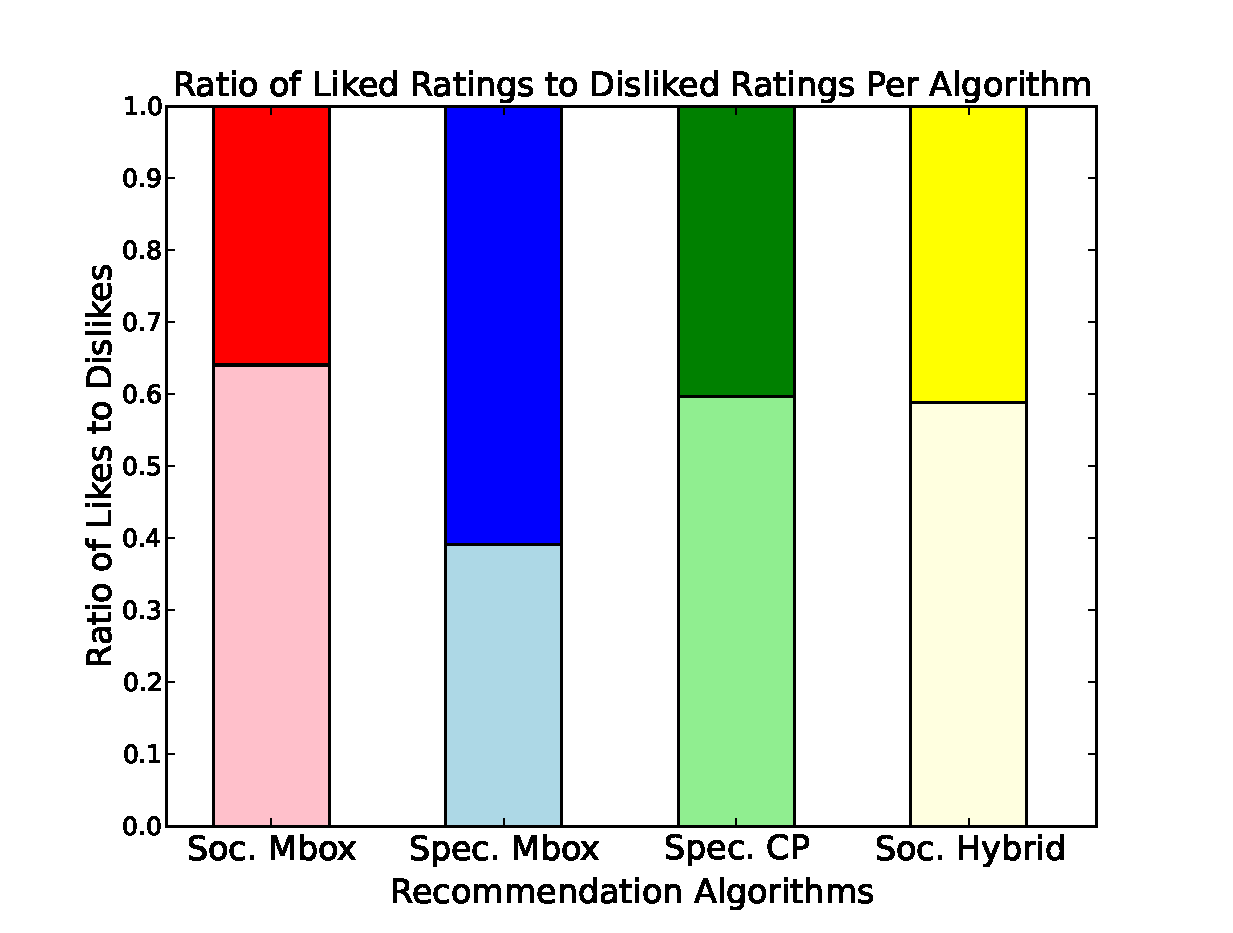
\includegraphics[scale=0.35]{img/live-likes2.eps}}
\subfigure{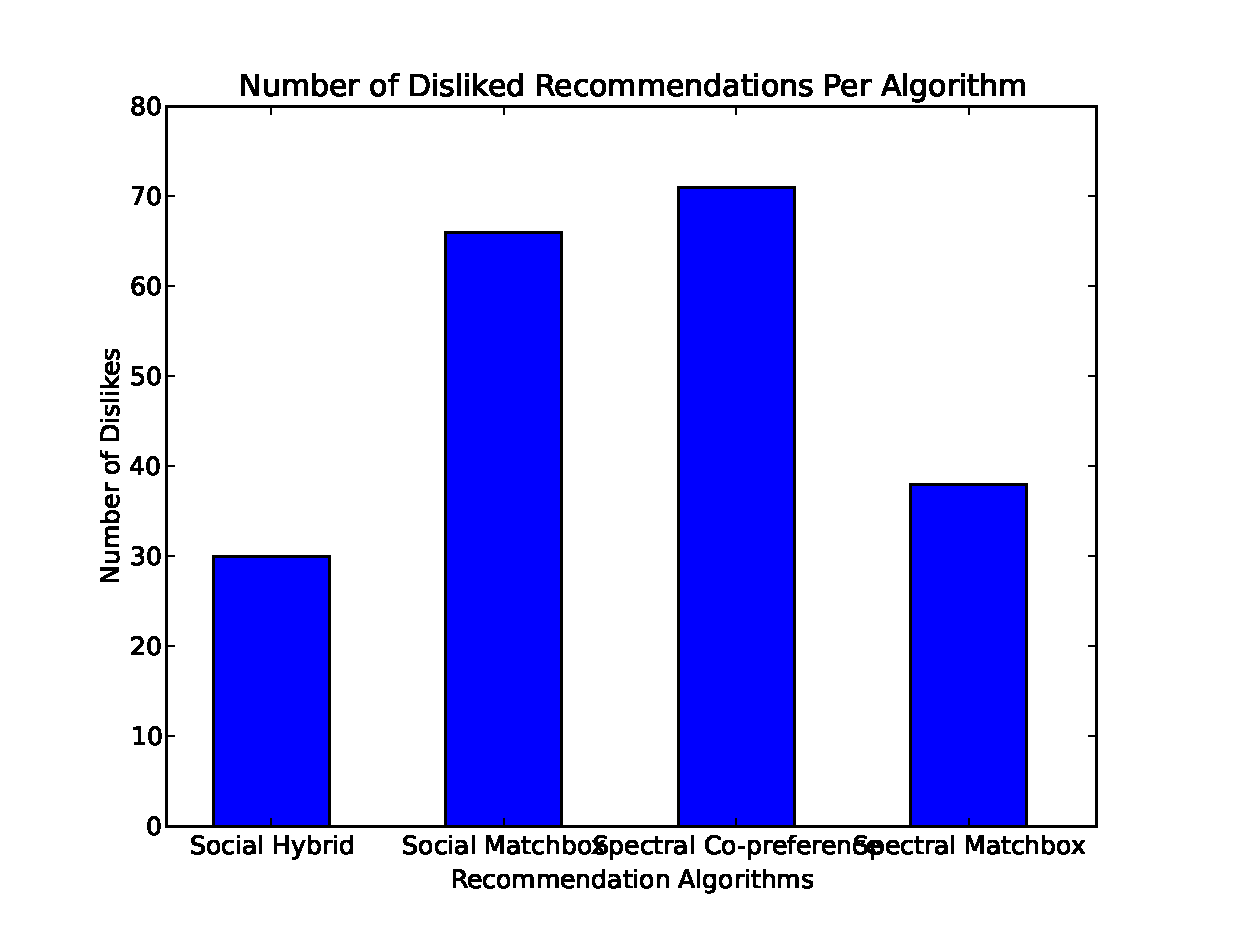
\includegraphics[scale=0.35]{img/live-dislikes2.eps}}
\caption{Results of online live trials. Spectral Matchbox achieved the highest ratio of likes to dislikes among the four algorithms.}
\end{figure}

We again split the results again between friend link recommendations and non-friend link recommendations, with the results shown being the number of likes or dislikes from friends or non-friends normalized by the total number of ratings on those type of recommendations. All four algorithms experiences a significant performance drop in the number of likes when it came to recommending non-friend links, which reflects the results of the first trial. Additionally, the differences were more drastic with the two algorithms that uses the social regularization method: Social Matchbox and Social Hybrid. This does seem to indeed show that aside from liking and disliking a link just from the quality of the links being recommended, users are also more likely to like a link simply because a friend had posted it and more likely to dislike it just because it came from a stranger.

\begin{figure}[h!]
\centering
\subfigure{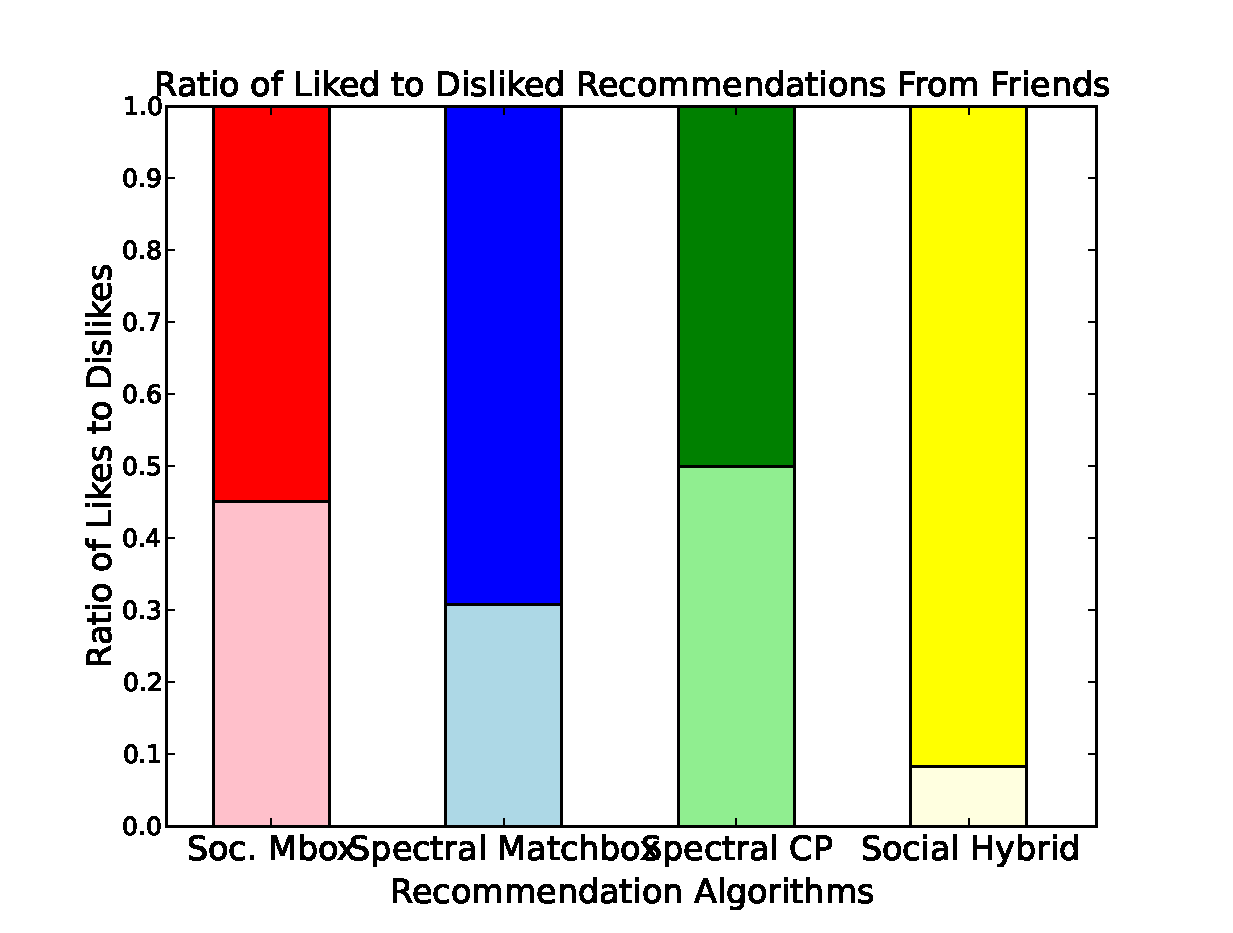
\includegraphics[scale=0.35]{img/live-friend-likes2.eps}}
\subfigure{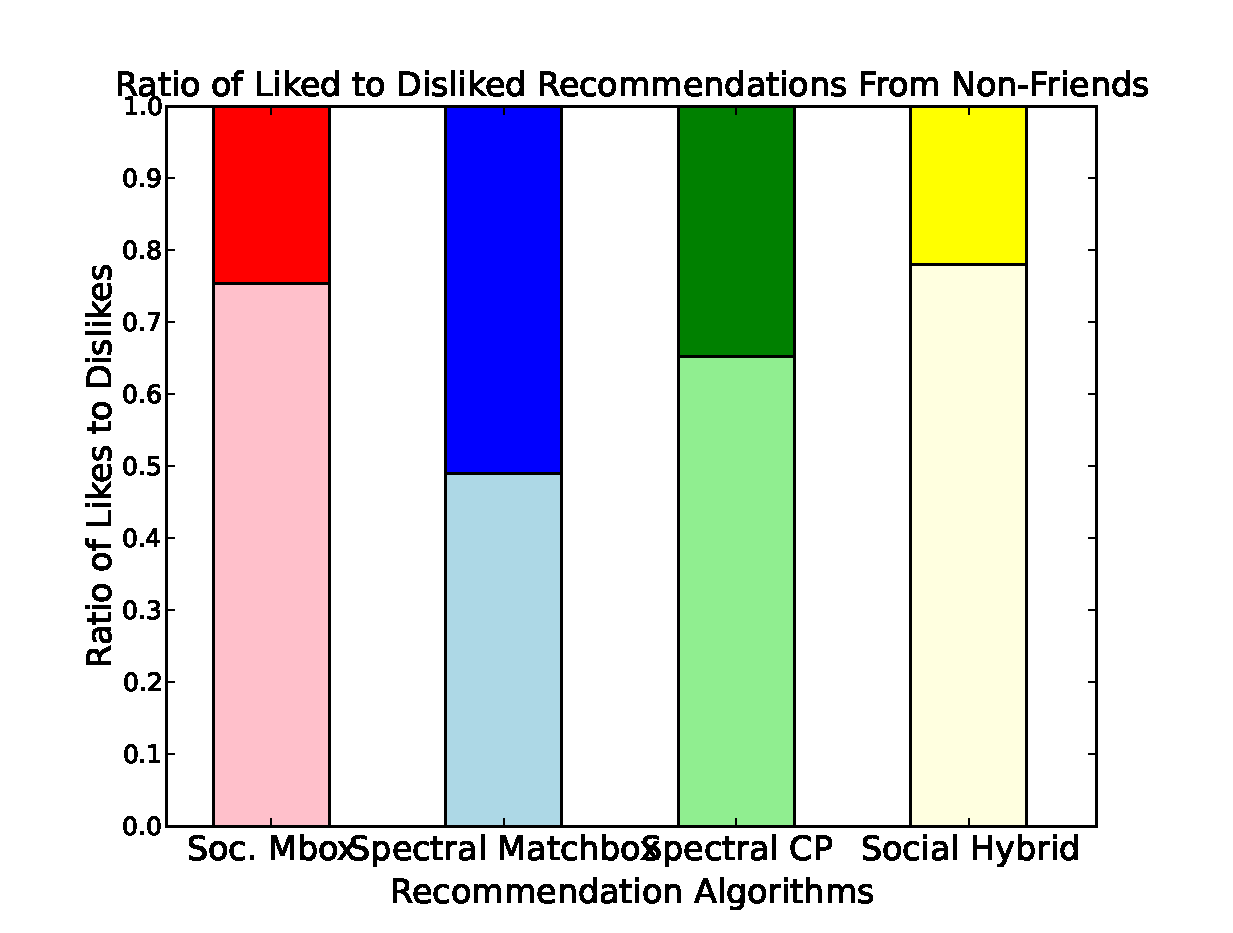
\includegraphics[scale=0.35]{img/live-nonfriend-likes2.eps}}
\subfigure{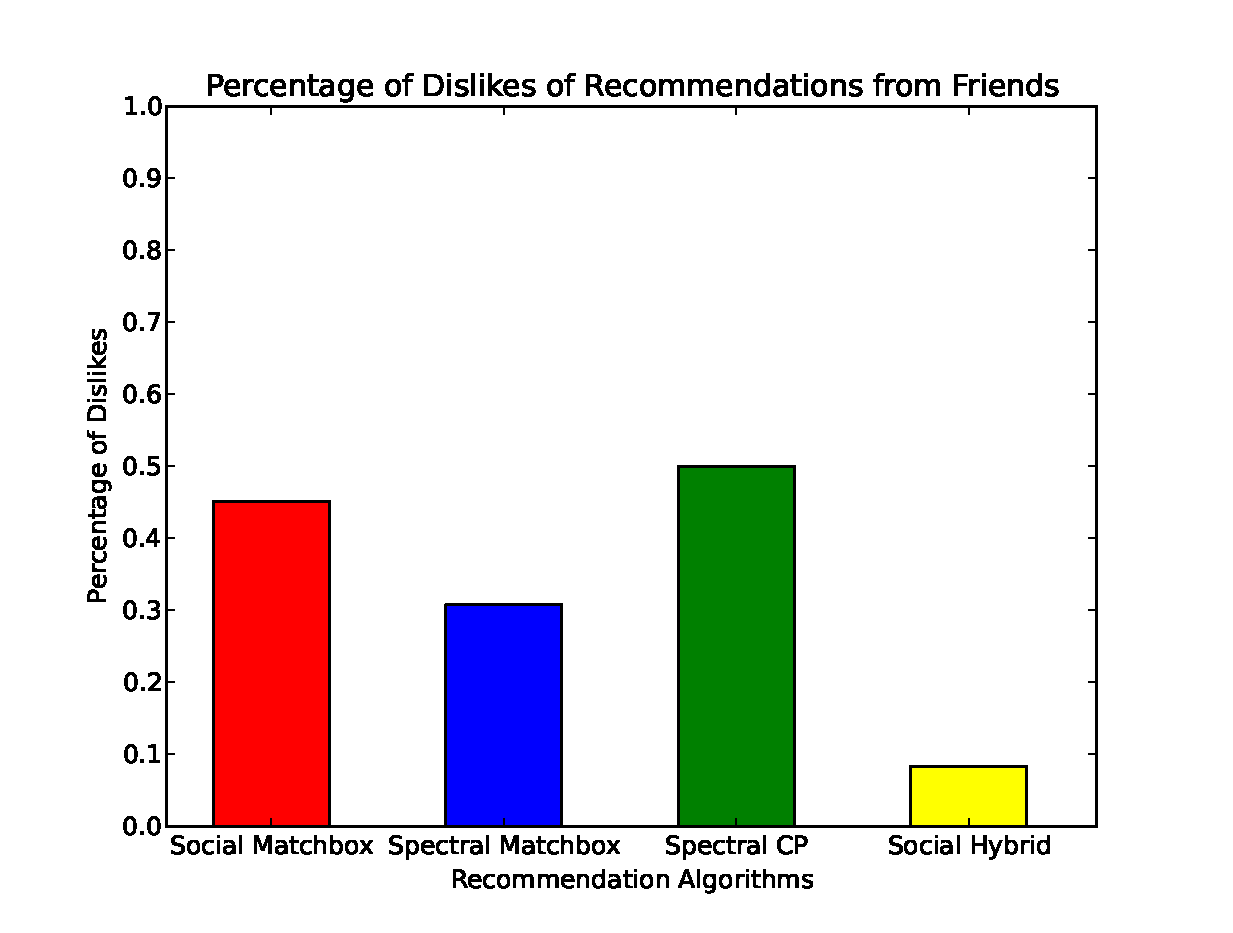
\includegraphics[scale=0.35]{img/live-friend-dislikes2.eps}}
\subfigure{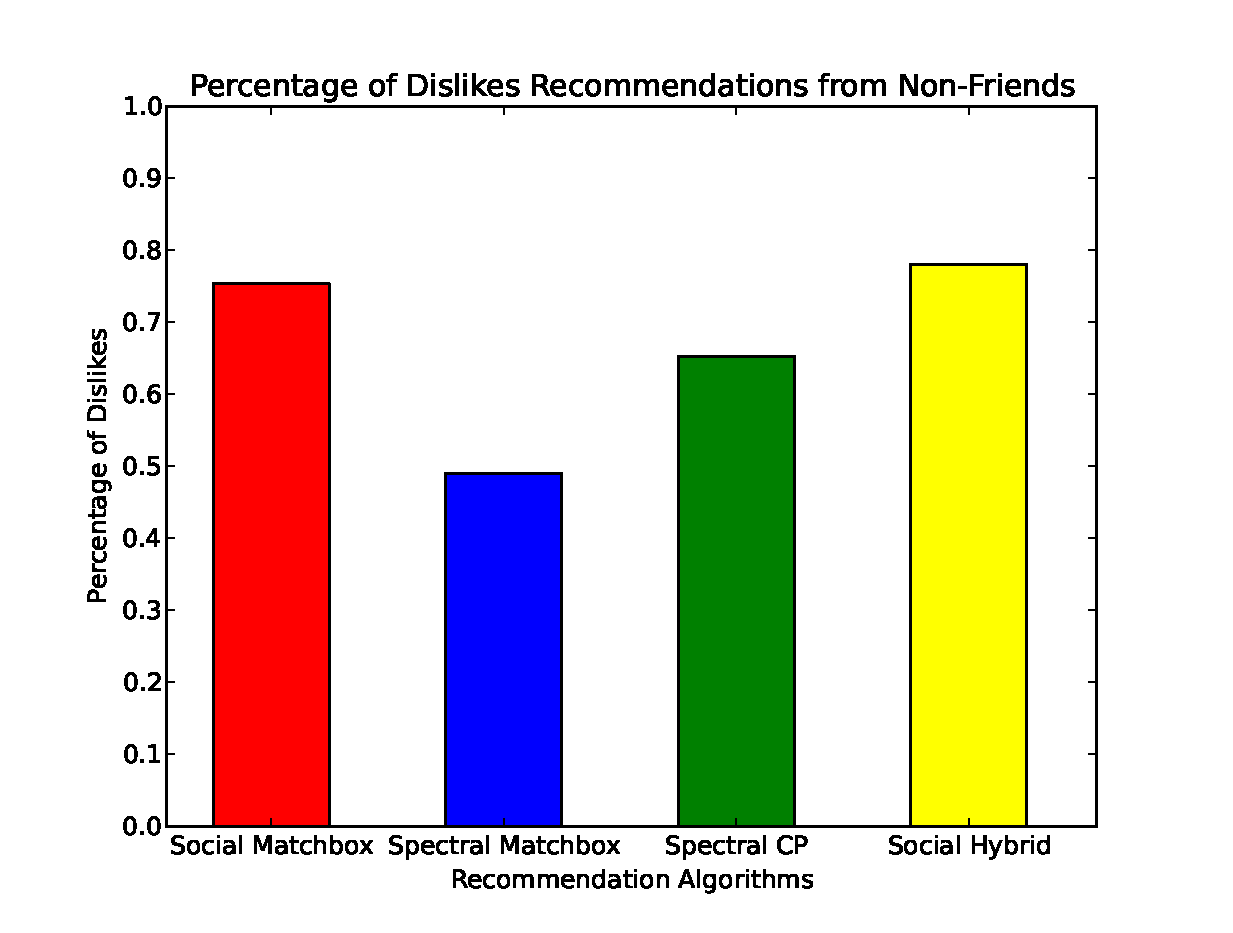
\includegraphics[scale=0.35]{img/live-nonfriend-dislikes2.eps}}
\caption{Results of the online live trials, split between friends and non-friends. As in the first trial, there is a significant drop in performance between recommending friend links and recommending non-friend links.}
\end{figure}

\section{Offline Results}

When testing on all the combinations of the active data, the results between the algorithms on a test dataset are all within the standard error bars. The results of the live trials aren't reflected in the offline results, which highlights the difficulty of using the MAP metric for evaluating recommendation algorithms offline.

%When training on the UNION dataset, we can see the same general worsening of performance between the results of testing on APP-USER-ACTIVE-FRIENDS and APP-USER-ACTIVE-NON-FRIENDS. 

\begin{figure}[h]
\centering
\subfigure{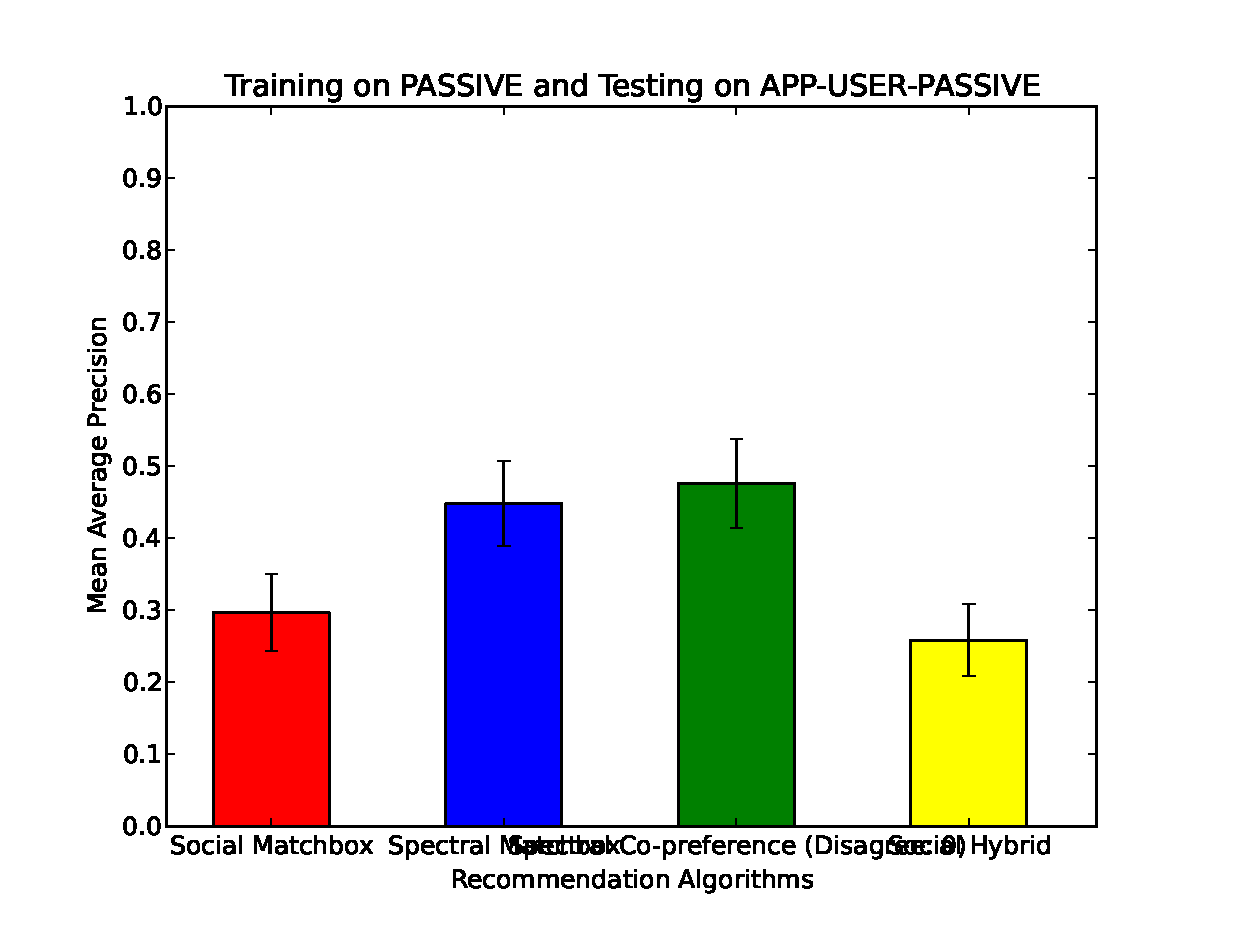
\includegraphics[scale=0.35]{img/Passive_App-User-Passive2.eps}}
\subfigure{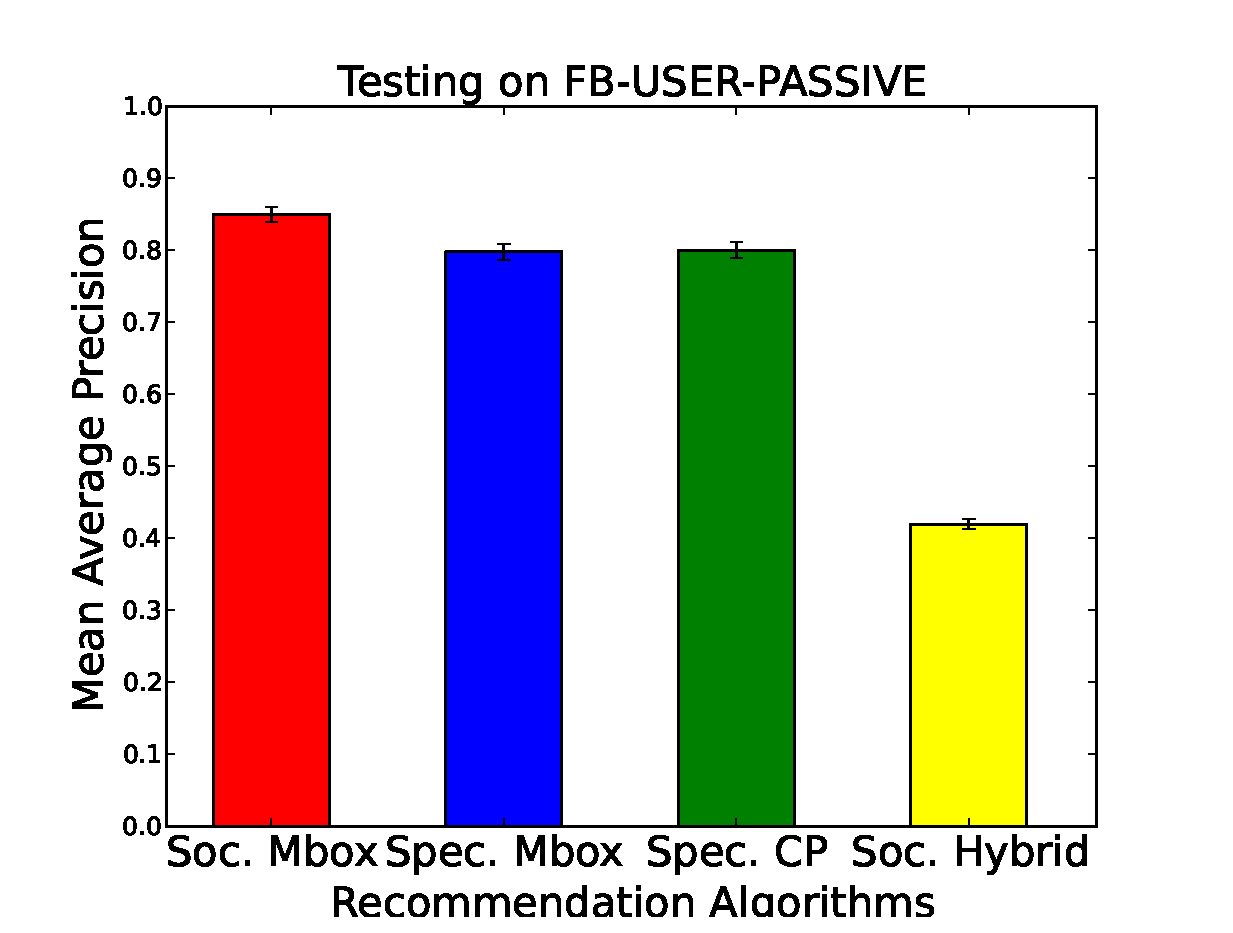
\includegraphics[scale=0.35]{img/Passive_FB-User-Passive2.eps}}
\subfigure{\includegraphics[scale=0.35]{img/Passive_App-User-active-all2.eps}}
\subfigure{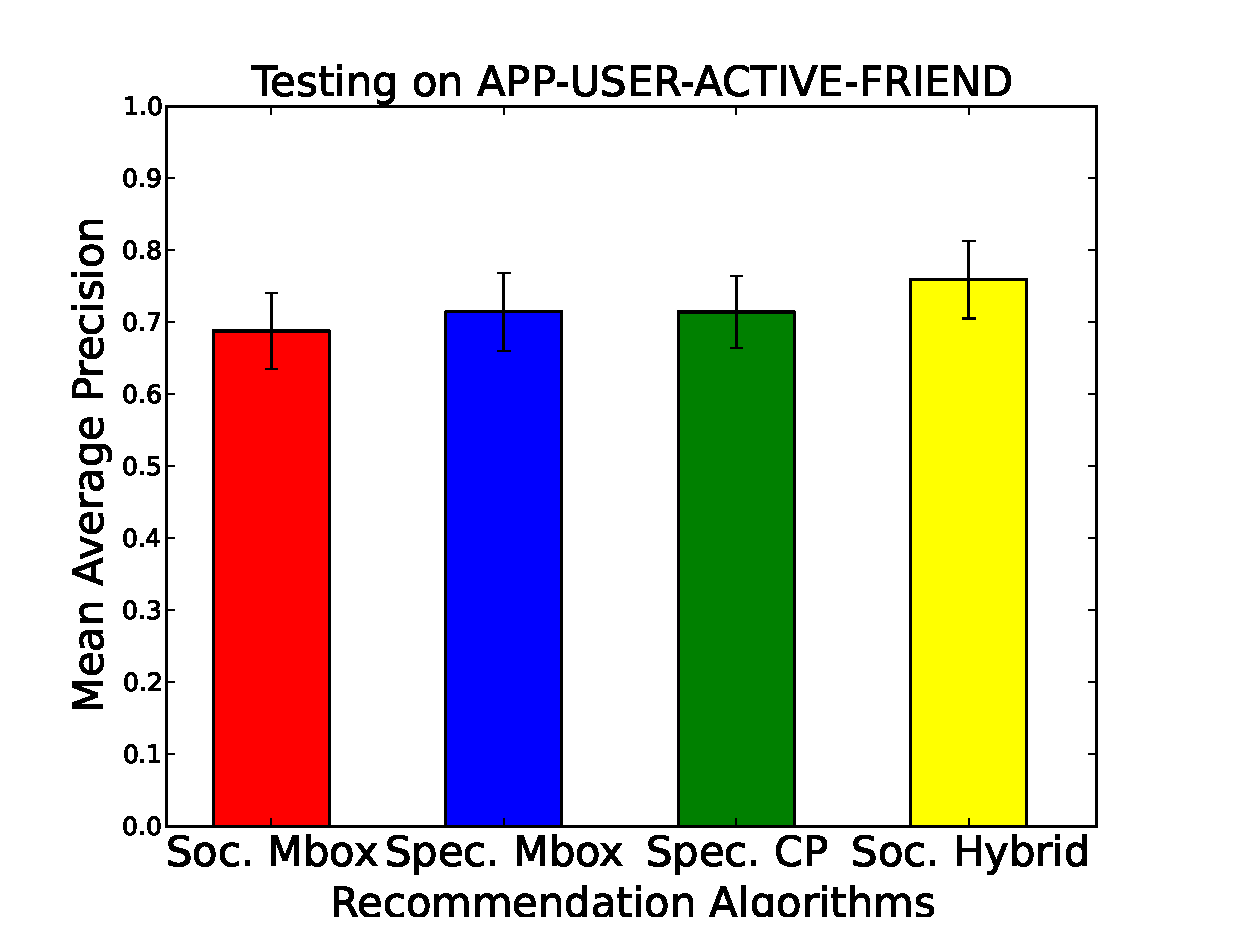
\includegraphics[scale=0.35]{img/Passive_App-User-Active-Friends2.eps}}
\subfigure{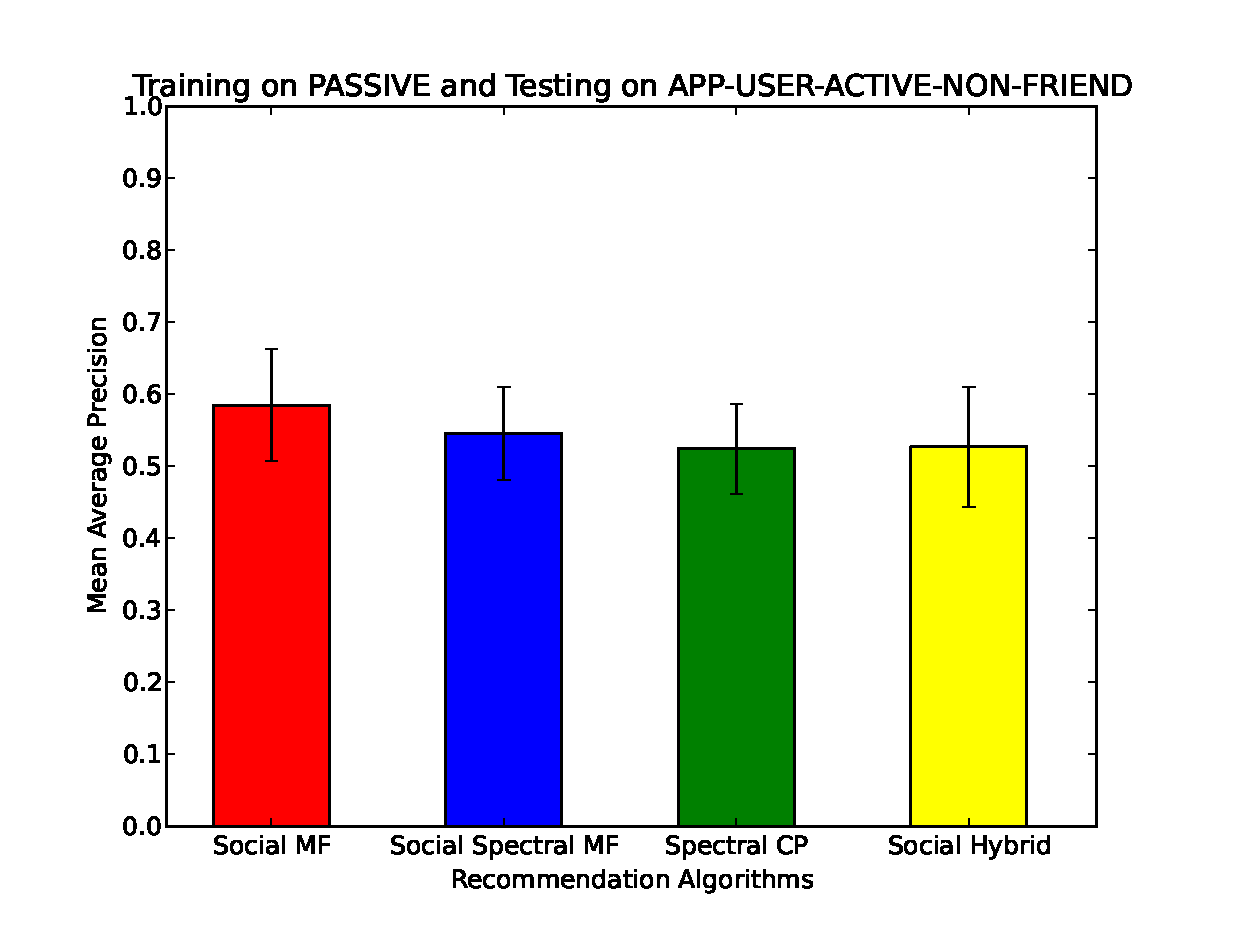
\includegraphics[scale=0.35]{img/Passive_App-User-Active-NonFriends2.eps}}
\caption{Results of training on Passive data}
\end{figure}

\begin{figure}[h]
\centering
\subfigure{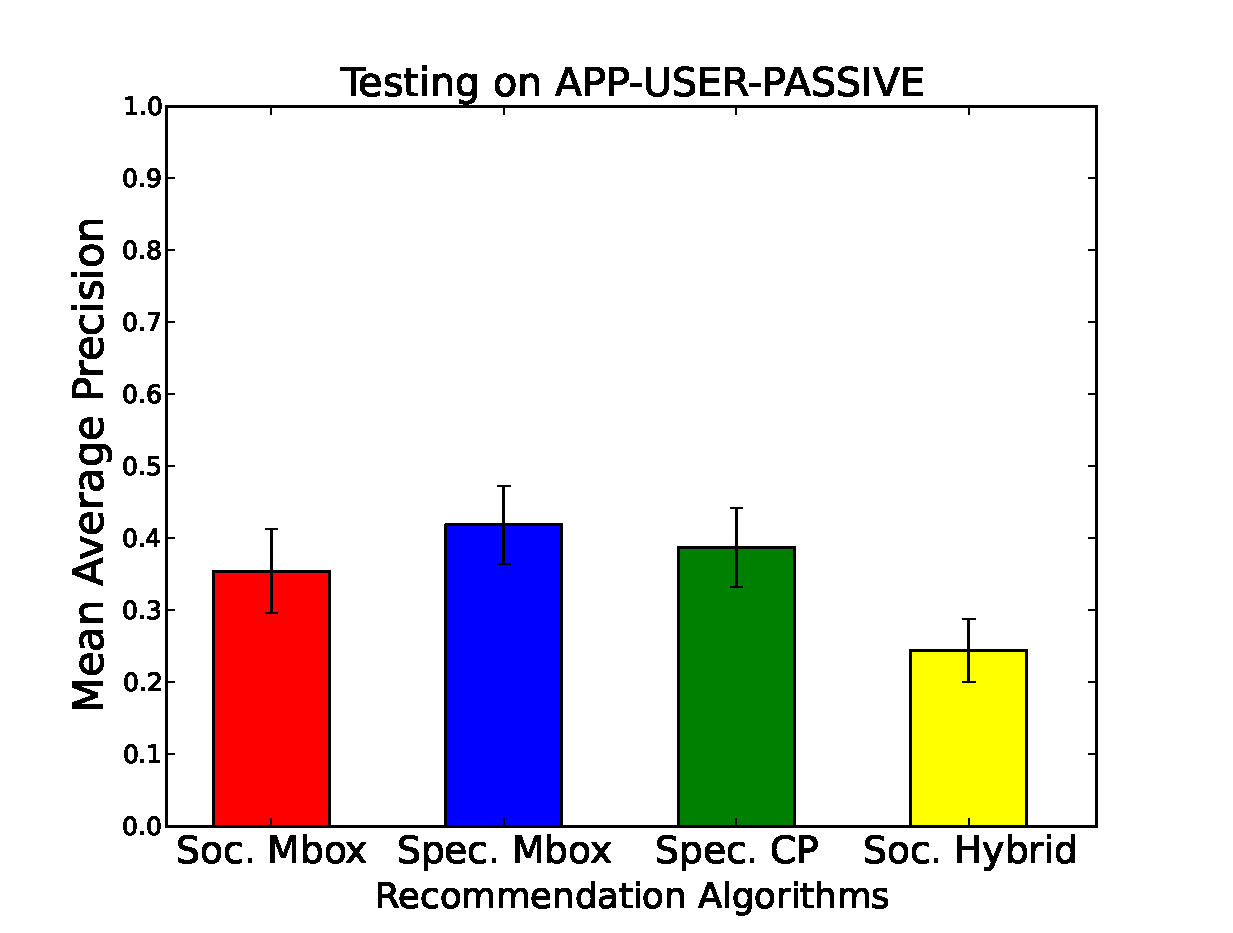
\includegraphics[scale=0.35]{img/Union_App-User-Passive2.eps}}
\subfigure{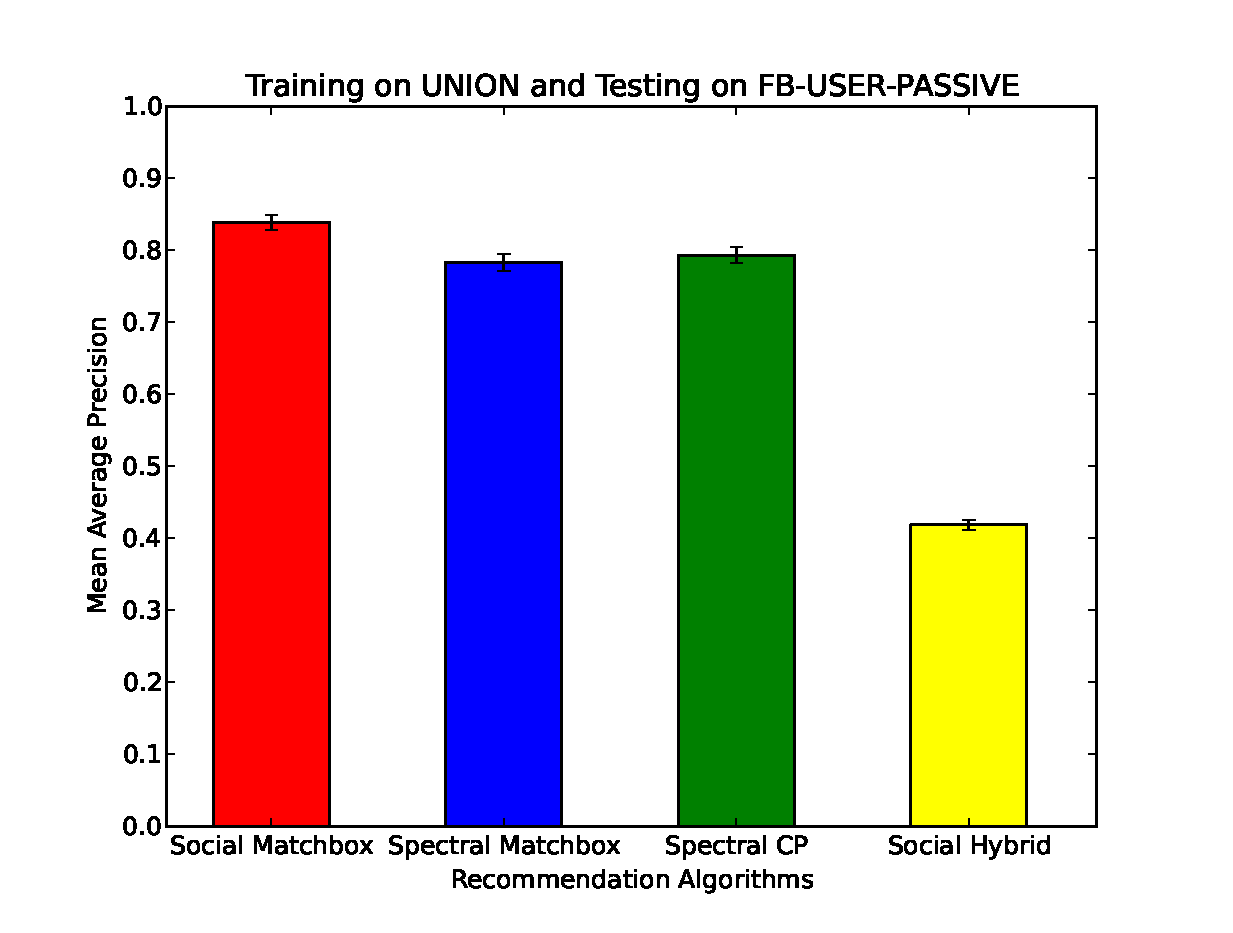
\includegraphics[scale=0.35]{img/Union_FB-User-Passive2.eps}}
\subfigure{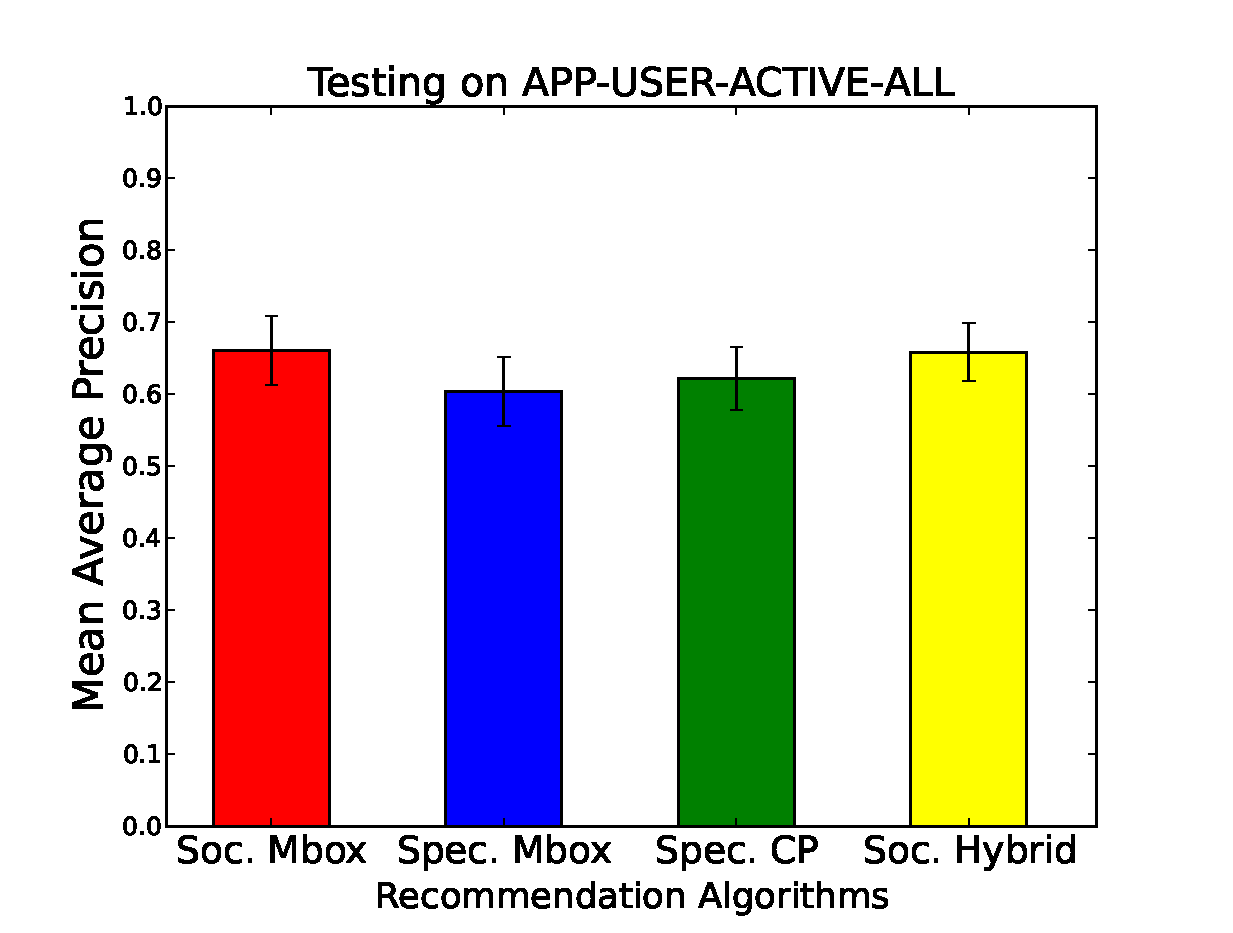
\includegraphics[scale=0.35]{img/Union_App-User-Active-All2.eps}}
\subfigure{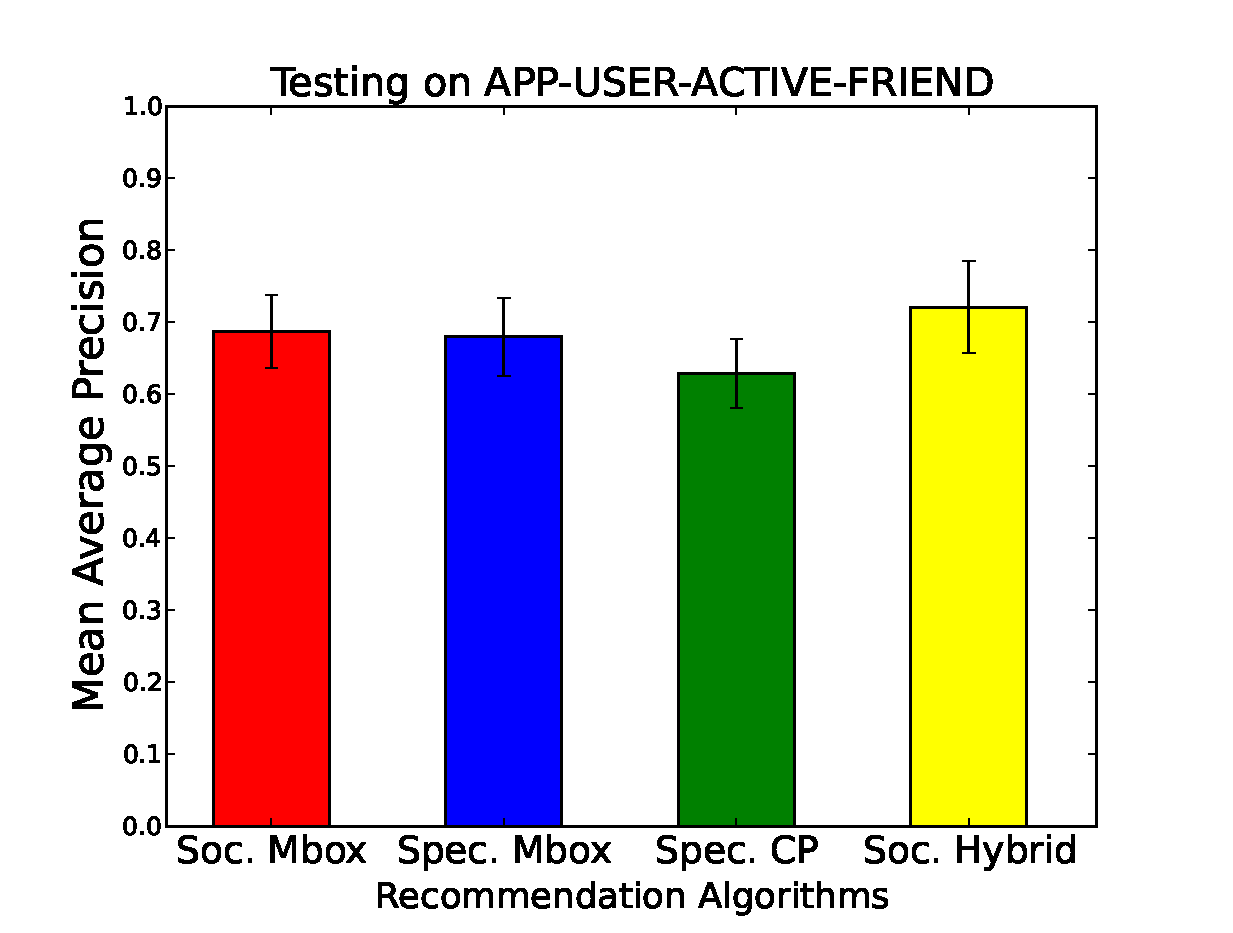
\includegraphics[scale=0.35]{img/Union_App-User-Active-Friends2.eps}}
\subfigure{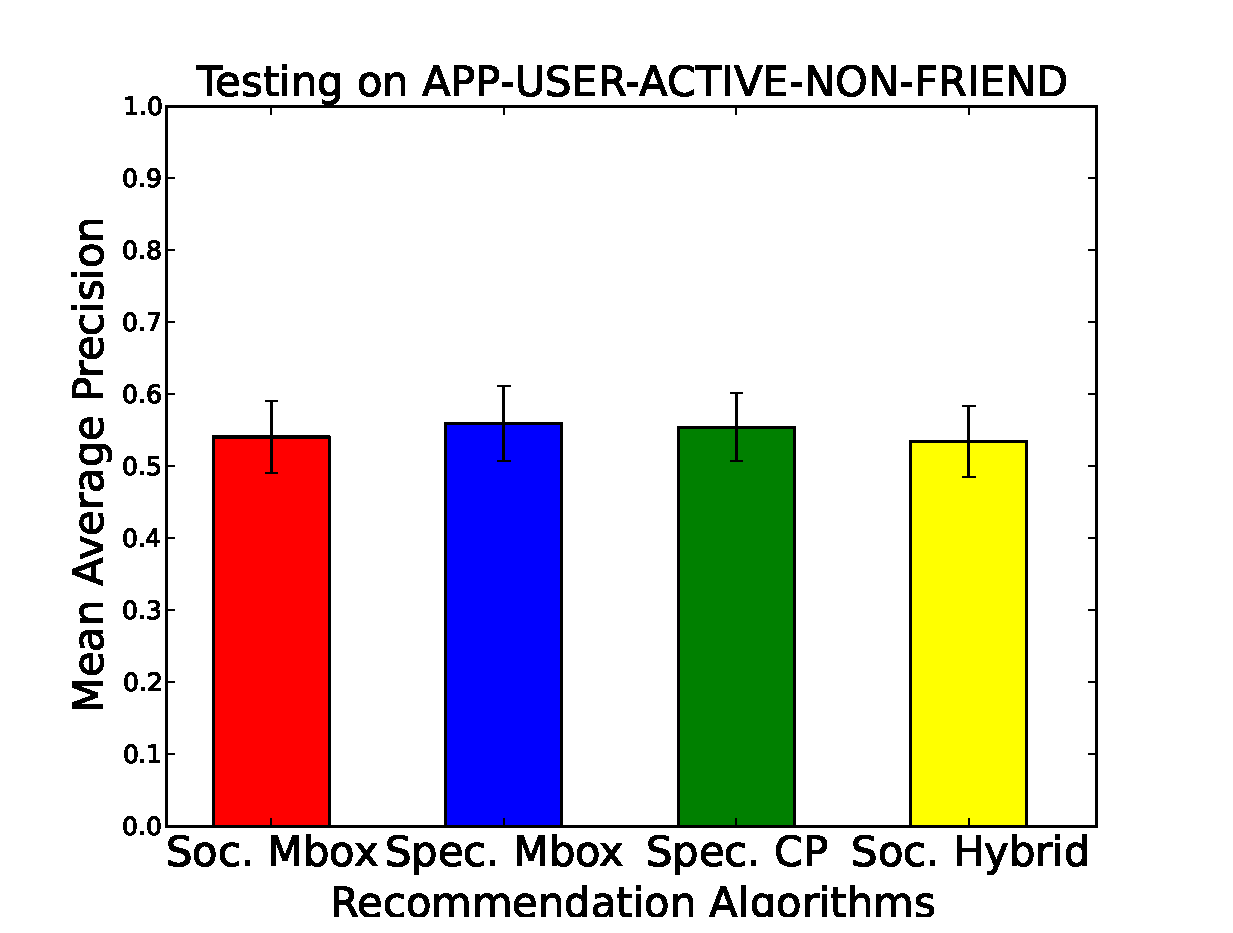
\includegraphics[scale=0.35]{img/Union_App-User-Active-NonFriends2.eps}}
\caption{Results of training on Union data}
\end{figure}

\begin{figure}[h]
\centering
\subfigure{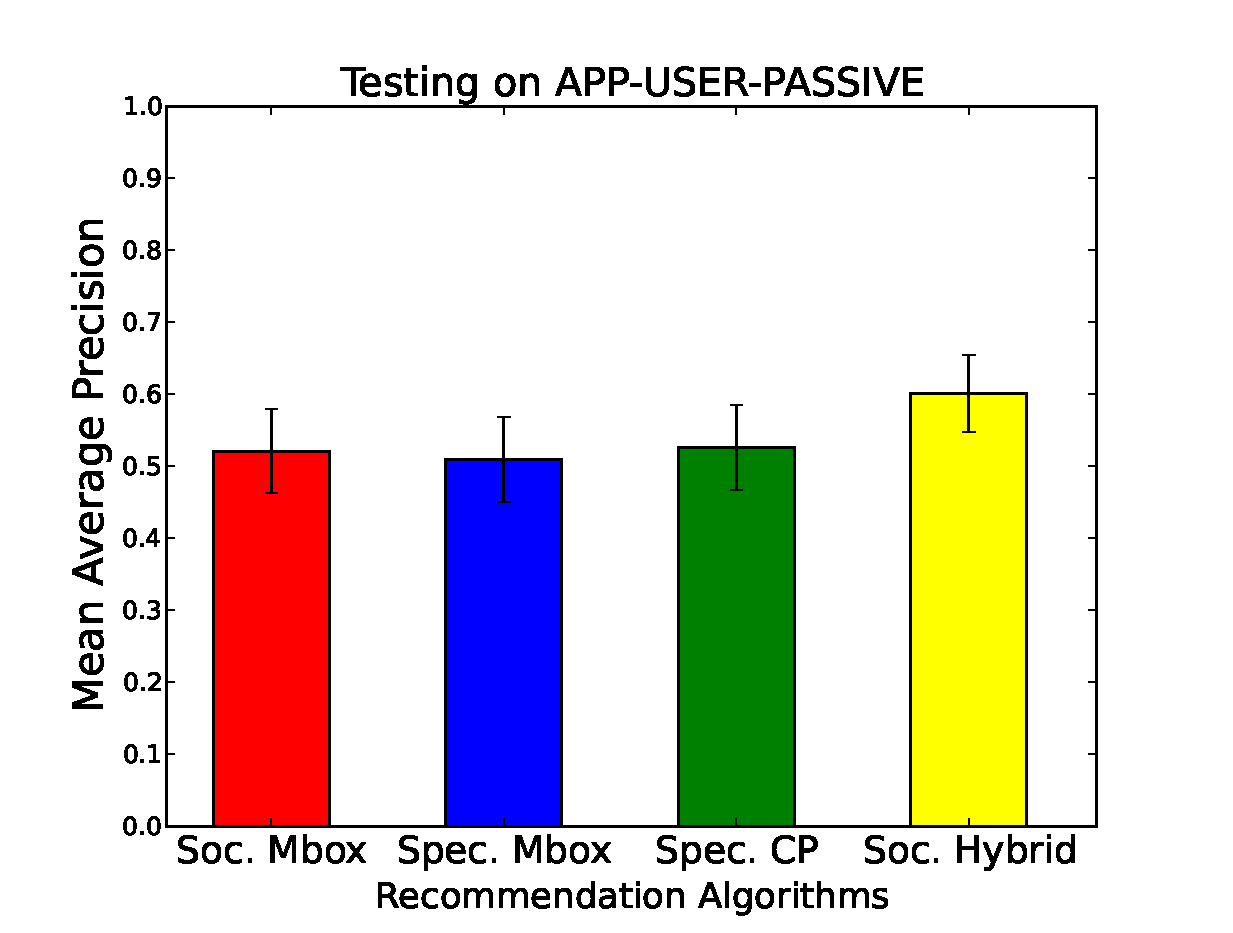
\includegraphics[scale=0.35]{img/Active_App-User-Passive2.eps}}
\subfigure{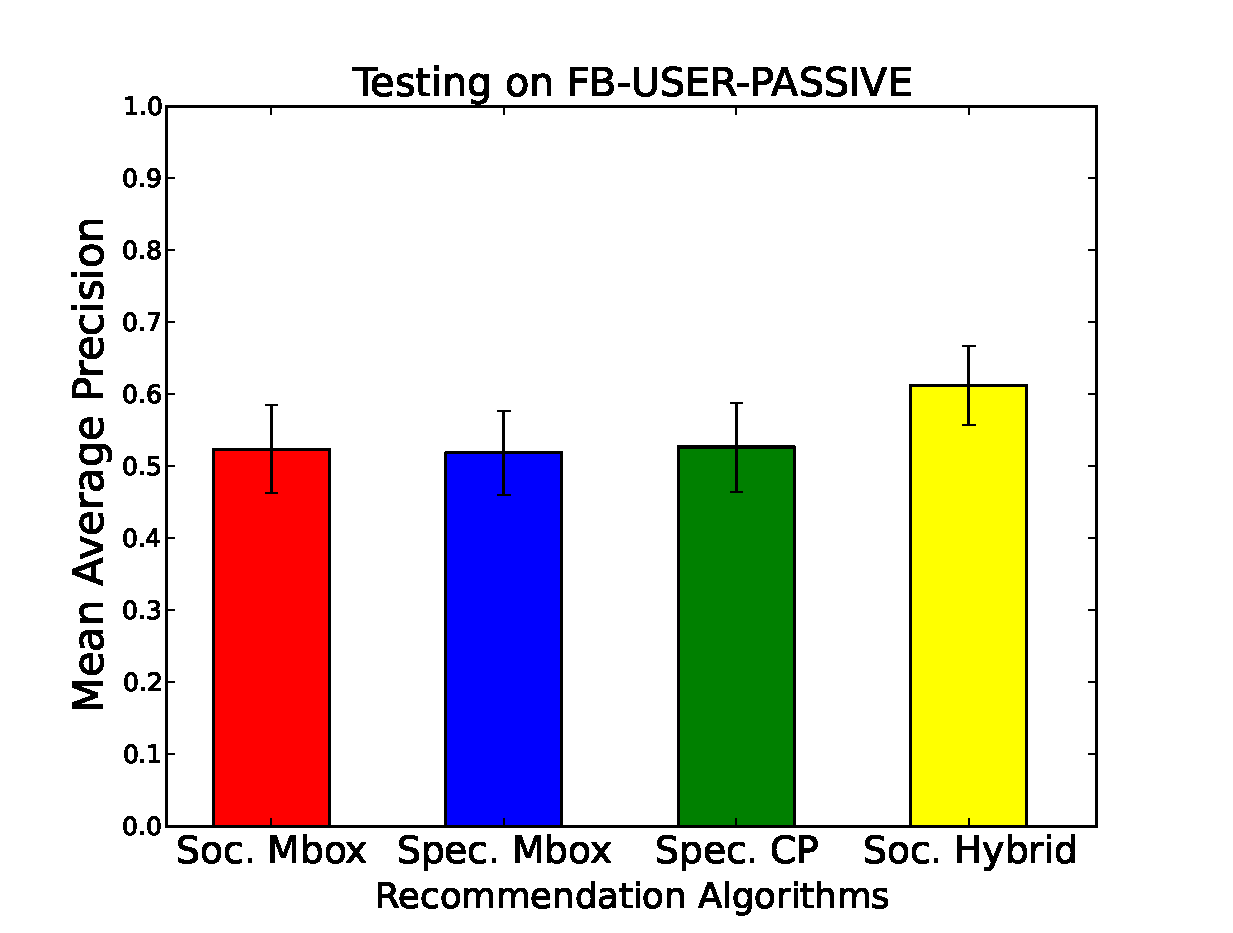
\includegraphics[scale=0.35]{img/Active_FB-User-Passive2.eps}}
\subfigure{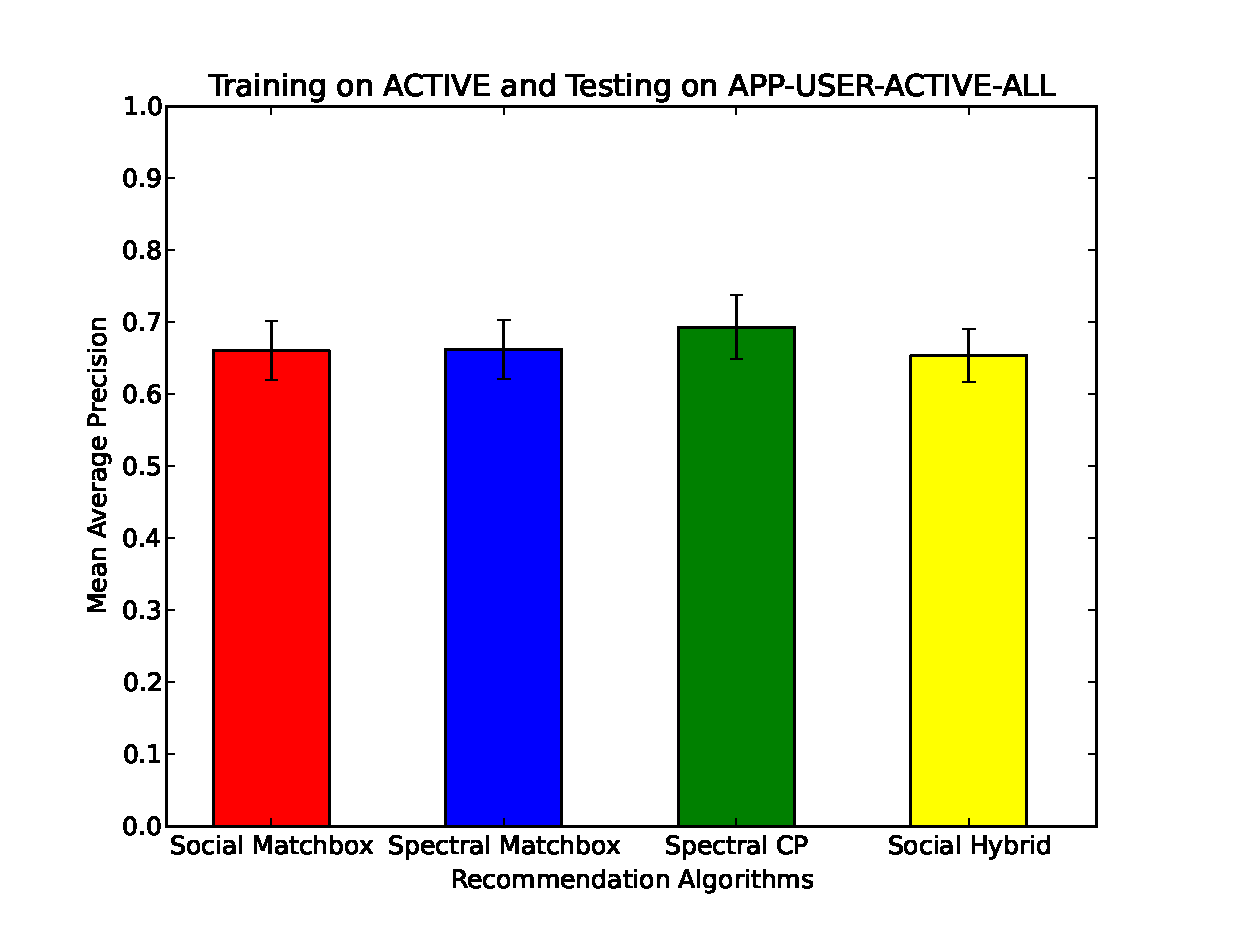
\includegraphics[scale=0.35]{img/Active_App-User-Active-All2.eps}}
\subfigure{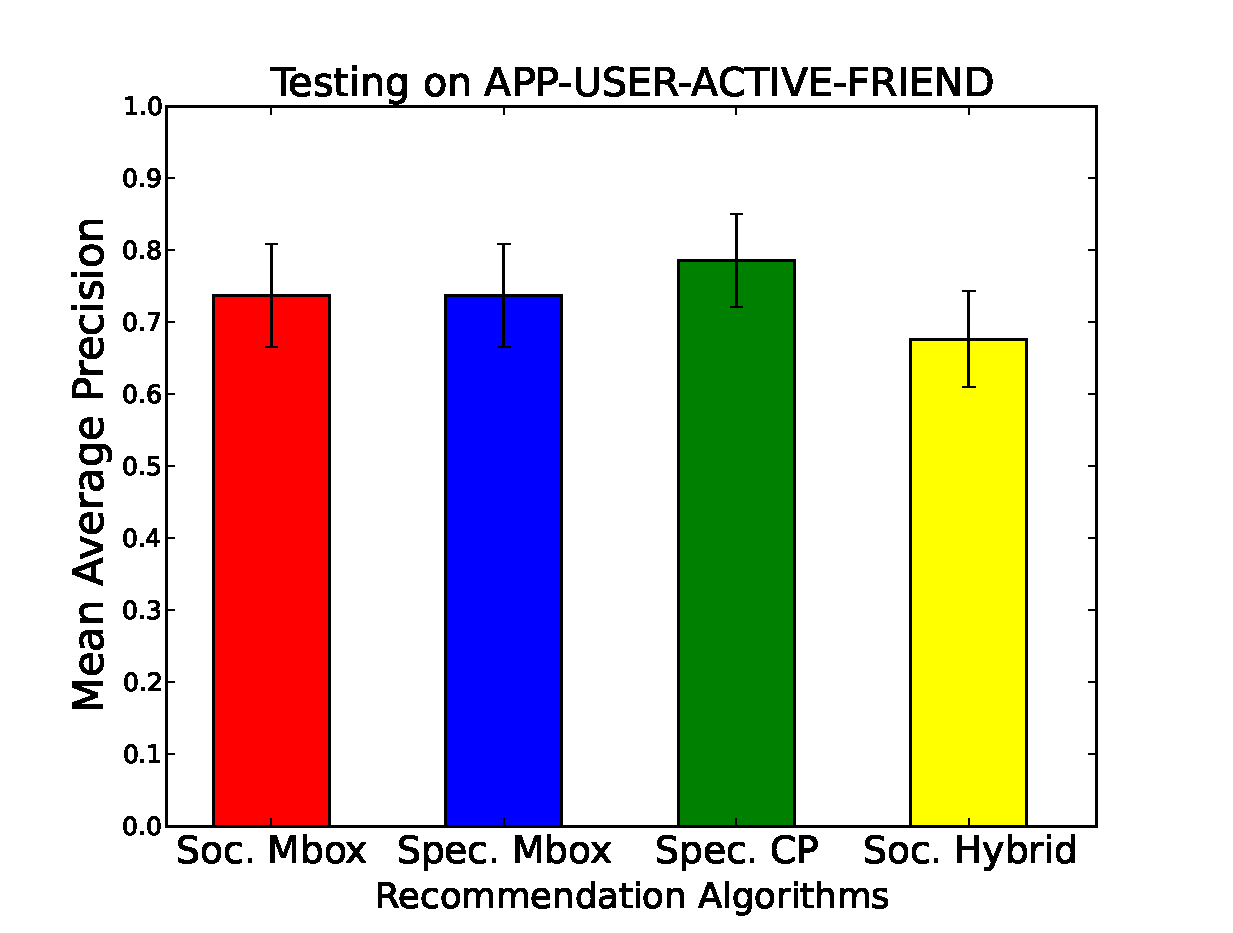
\includegraphics[scale=0.35]{img/Active_App-User-Active-Friends2.eps}}
\subfigure{\includegraphics[scale=0.35]{img/Active_App-User-Active-Nonfriends2.eps}}
\caption{Results of training on Active data}
\end{figure}
